\documentclass[12pt]{article}

\usepackage{booktabs}
\usepackage{tabularx}
\usepackage{float}
\usepackage{longtable}
\usepackage{array}
\usepackage{enumitem}
\usepackage{graphicx}
\usepackage{amssymb}
\usepackage{tikz}
\usetikzlibrary{positioning, arrows.meta}
\usepackage{fullpage} % same page setup as SRS-IEEE/SRS.tex

\title{Design Thinking Report\\\progname}

\author{\authname}

\date{}

% Common.text loads hyperref, so it goes last.
\input{../../Comments.text}
\input{../../Common.text}

%% ---------------------------------------------------------------------------
%% Design Thinking helper macros
%% ---------------------------------------------------------------------------

% Cross-reference helpers (same style as the Hazard Analysis).
% \partref{P01} links to the interview subsection labelled sec:P01.
\newcommand{\partref}[1]{\hyperref[sec:#1]{#1}}
% \ideaRef{A1} links to an idea in the Idea Generator.
\newcommand{\ideaRef}[1]{\hyperref[tab:IdeaGenerator]{#1}}

% Empathy map: a 2x2 grid of Say / Think / Do / Feel.
% Usage: \empathymap{<who>}{<say>}{<think>}{<do>}{<feel>}
% Each quadrant takes an itemize list or plain text.
\newcommand{\empathymap}[5]{%
  \begin{center}
  \renewcommand{\arraystretch}{1.3}
  \begin{tabularx}{\textwidth}{|>{\raggedright\arraybackslash}X|>{\raggedright\arraybackslash}X|}
    \multicolumn{2}{c}{\textbf{Empathy Map --- #1}}\\
    \hline
    \textbf{Say} \newline \footnotesize\emph{What they said, in answer to questions or unprompted.} \normalsize #2
    &
    \textbf{Think} \newline \footnotesize\emph{What we infer about their knowledge or opinions.} \normalsize #3
    \\ \hline
    \textbf{Do} \newline \footnotesize\emph{The steps they take to do the task we want to improve.} \normalsize #4
    &
    \textbf{Feel} \newline \footnotesize\emph{What we infer about their feelings, e.g.\ toward a proposed solution.} \normalsize #5
    \\ \hline
  \end{tabularx}
  \end{center}}

% Feedback grid: a 2x2 grid of Liked / Change / Questions / Ideas.
% Usage: \feedbackgrid{<who>}{<liked>}{<change>}{<questions>}{<ideas>}
\newcommand{\feedbackgrid}[5]{%
  \begin{center}
  \renewcommand{\arraystretch}{1.3}
  \begin{tabularx}{\textwidth}{|>{\raggedright\arraybackslash}X|>{\raggedright\arraybackslash}X|}
    \multicolumn{2}{c}{\textbf{Feedback Grid --- #1}}\\
    \hline
    \textbf{(+) Liked} \newline \footnotesize\emph{What did they like about it?} \normalsize #2
    &
    \textbf{($\Delta$) Change} \newline \footnotesize\emph{What would they like changed?} \normalsize #3
    \\ \hline
    \textbf{(?) Questions} \newline \footnotesize\emph{What questions did they ask?} \normalsize #4
    &
    \textbf{(!) Ideas} \newline \footnotesize\emph{What new ideas came out of the discussion?} \normalsize #5
    \\ \hline
  \end{tabularx}
  \end{center}}

% Interview skills self-assessment. Use \sel{...} to mark the option chosen.
\newcommand{\sel}[1]{\fbox{\textbf{#1}}}

% Let long table cells stretch instead of overflowing.
\setlength{\emergencystretch}{3em}

\begin{document}

\maketitle
\thispagestyle{empty}

~\newpage

\pagenumbering{roman}

\begin{table}[hp]
\caption{Revision History} \label{TblRevisionHistory}
\begin{tabularx}{\textwidth}{llX}
\toprule
\textbf{Date} & \textbf{Developer(s)} & \textbf{Change}\\
\midrule
Date1 & Name(s) & Description of changes\\
Date2 & Name(s) & Description of changes\\
... & ... & ...\\
\bottomrule
\end{tabularx}
\end{table}

\newpage

\tableofcontents

\listoftables

\listoffigures

\newpage

\pagenumbering{arabic}

%% ===========================================================================
\section{Introduction} \label{SecIntro}
%% ===========================================================================

\plt{This report documents the Design Thinking (DT) custom document for the
Fall term. It follows the steps of the DT worksheet from tutorial T03:
prepare, interview, ideate, prototype, get feedback, and reflect. The raw
worksheet slides (.pptx and .pdf) are also committed alongside this file
(Appendix~\ref{SecWorksheets}).}

\subsection{Purpose} \label{SecPurpose}

\plt{Why the team did Design Thinking: to understand the people \progname{} is
for, and their current way of tracking fitness and learning about investing,
before committing to requirements.}

\subsection{Scope} \label{SecScope}

\plt{What this report covers, and what it does not. The course asks for the
interview, ideation and two prototype stages only (the ``Design the Right
Thing'' diamond plus first prototypes), not the full DT process.}

\subsection{Design Thinking Process} \label{SecProcess}

\plt{Briefly describe the Double Diamond (Discover, Define, Develop, Deliver)
and map each section of this report to its phase. Keep or edit the figure
below.}

\begin{figure}[H]
\centering
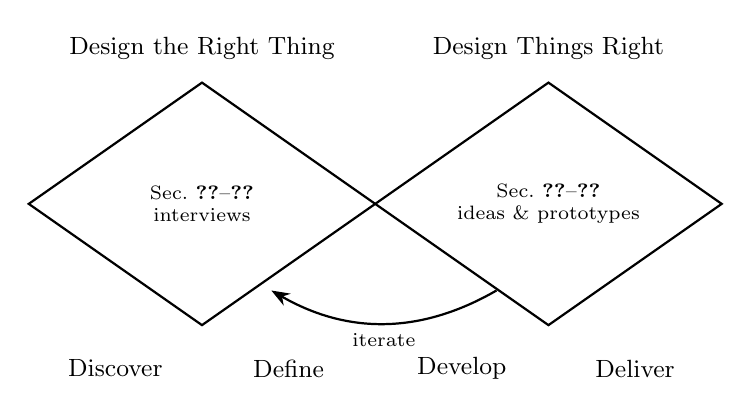
\begin{tikzpicture}[scale=1.1, every node/.style={font=\small}]
  \draw[thick] (0,0) -- (2,1.4) -- (4,0) -- (2,-1.4) -- cycle;
  \draw[thick] (4,0) -- (6,1.4) -- (8,0) -- (6,-1.4) -- cycle;
  \node at (2,1.8) {Design the Right Thing};
  \node at (6,1.8) {Design Things Right};
  \node at (1,-1.9) {Discover};
  \node at (3,-1.9) {Define};
  \node at (5,-1.9) {Develop};
  \node at (7,-1.9) {Deliver};
  \node[align=center, font=\scriptsize] at (2,0) {Sec.~\ref{SecPrep}--\ref{SecInterviews}\\interviews};
  \node[align=center, font=\scriptsize] at (6,0) {Sec.~\ref{SecIdeation}--\ref{SecFeedback}\\ideas \& prototypes};
  \draw[-{Stealth}, thick] (5.4,-1.0) to[bend left=30] node[below, font=\scriptsize]{iterate} (2.8,-1.0);
\end{tikzpicture}
\caption{The Double Diamond and where each section of this report fits}
\label{FigDoubleDiamond}
\end{figure}

\subsection{Relation to Other Documents} \label{SecRelatedDocs}

\plt{Which documents use the DT findings: SRS Section~3 (Stakeholder
Requirements) and Section~4 (User Personas), and V\&V Plan Section~3
(Custom Documents) and validation. Section~\ref{SecTrace} gives the full
traceability.}

\subsection{Participant Identifiers} \label{SecIDs}

\plt{Participants are referred to only by ID (P01, P02, \ldots), as in the SRS.
List each ID with a non-identifying description (e.g.\ ``university student,
tracks runs with a phone app'') and the interview date.}

\begin{table}[H]
\centering
\caption{Interview participants}
\label{TblParticipants}
\begin{tabularx}{\textwidth}{llX}
\toprule
\textbf{ID} & \textbf{Date} & \textbf{Description (non-identifying)}\\
\midrule
PP & Date & Practice interviewee (outside the team)\\
P01 & Oct 14, 2026 & \todo{description}\\
P02 & Oct 14, 2026 & \todo{description}\\
P03 & Date & \todo{optional third participant, or delete this row}\\
\bottomrule
\end{tabularx}
\end{table}

%% ===========================================================================
\section{Interview Preparation} \label{SecPrep}
%% ===========================================================================

\subsection{Target Users and Interview Goals} \label{SecTargetUsers}

\plt{Who the 2--3 potential users are (peers, the supervisor) and why they
were chosen. State the two goals from the worksheet: (1) understand the
problem, meaning their current day-to-day solution and its problems; and
(2) decide what value we can add without getting in the way of their current
routine.}

\subsection{Domain Research} \label{SecDomain}

\plt{Research done before the interviews, so we understand the fitness and
personal-finance domains. Answer the worksheet's questions below.}

\subsubsection{Usual Practices}
\plt{How people usually track fitness (phones, watches, apps), and how
beginners usually start investing (TFSAs, ETFs, paper trading, \ldots).}

\subsubsection{Common Problems}
\plt{Common problems people have in these domains (e.g.\ losing motivation,
fear of losing money, information overload).}

\subsubsection{Existing Solutions}

\begin{table}[H]
\centering
\caption{Existing solutions in the fitness and investing domains}
\label{TblExisting}
\begin{tabularx}{\textwidth}{lXX}
\toprule
\textbf{Product} & \textbf{What it does well} & \textbf{Gap \progname{} could fill}\\
\midrule
\todo{App 1} & & \\
\todo{App 2} & & \\
\todo{App 3} & & \\
\bottomrule
\end{tabularx}
\end{table}

\subsection{Introduction Script} \label{SecIntroScript}

\plt{What we say to an interviewee to explain why we are excited about this
problem area and why we need their help. Quote it word for word.}

\begin{quote}
\todo{Intro script}
\end{quote}

\subsection{Privacy and Ethics} \label{SecPrivacy}

\plt{How we protected participants: what we did \emph{not} collect, how
transcripts were de-identified (IDs only), consent, and no questions that
are too personal or unrelated to the problem, such as specific health
conditions or account balances.}

%% ===========================================================================
\section{Interview Questions} \label{SecQuestions}
%% ===========================================================================

\subsection{Initial Questions} \label{SecInitialQs}

\plt{Open-ended questions to guide the interview. Follow-up questions asked
during the interview should be written down too.}

\begin{enumerate}[label=Q\arabic*.]
  \item \todo{Question}
  \item \todo{Question}
  \item \todo{Question}
  \item \todo{Question}
  \item \todo{Question}
  \item \todo{Question}
  \item \todo{Question}
\end{enumerate}

\subsection{Practice Interview} \label{SecPractice}

\plt{Practice interview with someone outside the team, to ``debug'' the
questions. One or two people interview and at least two take notes.}

\subsubsection{Practice Notes}
\plt{Summary of what they said.}

\subsubsection{Practice Empathy Map}

\empathymap{Practice interviewee (PP)}
{\begin{itemize}[leftmargin=*,nosep] \item \todo{} \end{itemize}}
{\begin{itemize}[leftmargin=*,nosep] \item \todo{} \end{itemize}}
{\begin{itemize}[leftmargin=*,nosep] \item \todo{} \end{itemize}}
{\begin{itemize}[leftmargin=*,nosep] \item \todo{} \end{itemize}}

\subsubsection{Interview Skills Self-Assessment (Practice)}

\plt{Mark one option per row with \textbackslash sel\{\}.}

\begin{table}[H]
\centering
\caption{Interview skills self-assessment, practice interview}
\label{TblSkillsPractice}
\begin{tabularx}{\textwidth}{Xlll}
\toprule
\textbf{Did you\ldots} & \multicolumn{3}{c}{\textbf{Choose one}}\\
\midrule
Set up the interview, giving context? & Somewhat & Yes & Definitely!\\
Make them comfortable? & Somewhat & Yes & Definitely!\\
Ask open-ended questions? & Never & Sometimes & Whenever appropriate\\
Ask follow-ups? & Never & Sometimes & Whenever appropriate\\
Ask how they felt about things? & Never & Sometimes & Whenever appropriate\\
Ask for stories, or the steps of a task? & Never & Sometimes & Whenever appropriate\\
React to non-verbal cues? & Never & Sometimes & Always\\
\bottomrule
\end{tabularx}
\end{table}

\subsection{Revised Questions} \label{SecRevisedQs}

\plt{Questions after the practice run. Note what changed and why
(e.g.\ ``Q3 was too leading, so it was reworded'').}

\begin{enumerate}[label=Q\arabic*.]
  \item \todo{Question}
  \item \todo{Question}
  \item \todo{Question}
  \item \todo{Question}
  \item \todo{Question}
  \item \todo{Question}
  \item \todo{Question}
\end{enumerate}

%% ===========================================================================
\section{User Interviews} \label{SecInterviews}
%% ===========================================================================

\plt{One subsection per participant. Keep transcripts de-identified. Copy the
P01 block for each additional participant.}

\subsection{Participant P01} \label{sec:P01}

\subsubsection{Context}
\plt{Date, format (in person or online), interviewer(s), note-takers, and how
long it took.}

\subsubsection{Transcript Summary}
\plt{Key answers per question; short quotes are fine.}

\subsubsection{Empathy Map}

\empathymap{P01}
{\begin{itemize}[leftmargin=*,nosep] \item \todo{} \end{itemize}}
{\begin{itemize}[leftmargin=*,nosep] \item \todo{} \end{itemize}}
{\begin{itemize}[leftmargin=*,nosep] \item \todo{} \end{itemize}}
{\begin{itemize}[leftmargin=*,nosep] \item \todo{} \end{itemize}}

\subsection{Participant P02} \label{sec:P02}

\subsubsection{Context}
\plt{Date, format, interviewer(s), note-takers, and how long it took.}

\subsubsection{Transcript Summary}
\plt{Key answers per question.}

\subsubsection{Empathy Map}

\empathymap{P02}
{\begin{itemize}[leftmargin=*,nosep] \item \todo{} \end{itemize}}
{\begin{itemize}[leftmargin=*,nosep] \item \todo{} \end{itemize}}
{\begin{itemize}[leftmargin=*,nosep] \item \todo{} \end{itemize}}
{\begin{itemize}[leftmargin=*,nosep] \item \todo{} \end{itemize}}

\subsection{Participant P03 (Optional)} \label{sec:P03}

\plt{Delete this subsection if only two interviews were held. If we interview
a beginner investor, this closes the gap noted in the V\&V Plan.}

\subsection{Interview Skills Self-Assessment} \label{SecSkills}

\begin{table}[H]
\centering
\caption{Interview skills self-assessment, real interviews}
\label{TblSkills}
\begin{tabularx}{\textwidth}{Xlll}
\toprule
\textbf{Did you\ldots} & \multicolumn{3}{c}{\textbf{Choose one}}\\
\midrule
Set up the interview, giving context? & Somewhat & Yes & Definitely!\\
Make them comfortable? & Somewhat & Yes & Definitely!\\
Ask open-ended questions? & Never & Sometimes & Whenever appropriate\\
Ask follow-ups? & Never & Sometimes & Whenever appropriate\\
Ask how they felt about things? & Never & Sometimes & Whenever appropriate\\
Ask for stories, or the steps of a task? & Never & Sometimes & Whenever appropriate\\
React to non-verbal cues? & Never & Sometimes & Always\\
\bottomrule
\end{tabularx}
\end{table}

\subsection{Key Insights} \label{SecInsights}

\plt{Converge (the ``Define'' phase): the themes that came up across
participants. Give each insight an ID (I1, I2, \ldots) so later sections and
the SRS can trace to it.}

\begin{table}[H]
\centering
\caption{Key insights from the interviews}
\label{TblInsights}
\begin{tabularx}{\textwidth}{lXl}
\toprule
\textbf{ID} & \textbf{Insight} & \textbf{Source}\\
\midrule
I1 & \todo{Insight} & \partref{P01}, \partref{P02}\\
I2 & \todo{Insight} & \partref{P01}\\
I3 & \todo{Insight} & \partref{P02}\\
\bottomrule
\end{tabularx}
\end{table}

%% ===========================================================================
\section{Ideation} \label{SecIdeation}
%% ===========================================================================

\subsection{Idea Generator} \label{SecIdeaGen}

\plt{Structured brainstorming. Put two aspects of the problem on the axes
(e.g.\ user pain points from Section~\ref{SecInsights} $\times$ app areas or
user goals) and fill in \textbf{all 16 cells}, even if some ideas are crazy
or unrealistic.}

\begin{table}[H]
\centering
\caption{Idea Generator}
\label{tab:IdeaGenerator}
\renewcommand{\arraystretch}{1.4}
\begin{tabularx}{\textwidth}{|l|X|X|X|X|}
\hline
 & \textbf{A.} \todo{Aspect} & \textbf{B.} \todo{Aspect} & \textbf{C.} \todo{Aspect} & \textbf{D.} \todo{Aspect}\\
\hline
\textbf{1.} \todo{Aspect} & A1: & B1: & C1: & D1: \\ \hline
\textbf{2.} \todo{Aspect} & A2: & B2: & C2: & D2: \\ \hline
\textbf{3.} \todo{Aspect} & A3: & B3: & C3: & D3: \\ \hline
\textbf{4.} \todo{Aspect} & A4: & B4: & C4: & D4: \\ \hline
\end{tabularx}
\end{table}

\subsection{Desirability vs.\ Feasibility} \label{SecDvF}

\plt{As a group, go through the ideas in reverse order and score each one
from 1 to 10. Feasibility: how possible it is to build with our resources.
Desirability: how much impact it would have on the user, supervisor or client.
The best ideas end up near the top-right of the plot.}

\begin{table}[H]
\centering
\caption{Desirability and feasibility scores}
\label{TblDvF}
\begin{tabular}{lccl}
\toprule
\textbf{Idea} & \textbf{Desirability (1--10)} & \textbf{Feasibility (1--10)} & \textbf{Notes}\\
\midrule
A1 & & & \\
\ldots & & & \\
D4 & & & \\
\bottomrule
\end{tabular}
\end{table}

\begin{figure}[H]
\centering
\begin{tikzpicture}[scale=0.55]
  \draw[-{Stealth}] (0,0) -- (10.5,0);
  \node[font=\small] at (5,-1.3) {Desirability};
  \draw[-{Stealth}] (0,0) -- (0,10.5);
  \node[font=\small, rotate=90] at (-1.4,5) {Feasibility};
  \foreach \t in {2,4,6,8,10} {
    \draw (\t,0.1) -- (\t,-0.1) node[below, font=\scriptsize]{\t};
    \draw (0.1,\t) -- (-0.1,\t) node[left, font=\scriptsize]{\t};
  }
  \draw[dashed, gray] (5,0) -- (5,10);
  \draw[dashed, gray] (0,5) -- (10,5);
  % Plot each idea as: \node[idea] at (desirability, feasibility) {ID};
  \tikzset{idea/.style={circle, fill=cyan!25, draw, inner sep=1pt, font=\scriptsize}}
  \node[idea] at (8,7) {A1}; % EXAMPLE: replace with real scores
\end{tikzpicture}
\caption{Desirability vs.\ feasibility of each idea}
\label{FigDvF}
\end{figure}

\subsection{Selected Ideas} \label{SecSelected}

\plt{The two best ideas, which become Prototype~1 and Prototype~2. For each
one, say why it was chosen (its scores and the insights it addresses) and
what we want to learn from testing it.}

\begin{description}
  \item[Prototype 1 (\ideaRef{XX}):] \todo{idea, rationale, what we hope to learn}
  \item[Prototype 2 (\ideaRef{XX}):] \todo{idea, rationale, what we hope to learn}
\end{description}

\subsection{Discussion Points} \label{SecDiscussion}

\plt{Questions raised by this process that we parked for later, e.g.\ parts of
what we learned that we don't yet know how to build.}

%% ===========================================================================
\section{Prototypes} \label{SecPrototypes}
%% ===========================================================================

\plt{Low-fidelity (paper or tablet) prototypes. Focus on how they work, not
how they look; give users enough to react to. Put images in
\texttt{figures/} and add one figure per screen or action.}

\subsection{Prototype 1: \todo{Name}} \label{SecProto1}

\plt{Describe the flow, then add the screens.}

% \begin{figure}[H]
%   \centering
%   \includegraphics[width=0.45\textwidth]{figures/proto1_screen1.png}
%   \caption{Prototype 1 --- Screen 1}
%   \label{FigProto1S1}
% \end{figure}

\subsection{Prototype 2: \todo{Name}} \label{SecProto2}

\plt{Describe the flow, then add the screens.}

%% ===========================================================================
\section{Prototype Feedback} \label{SecFeedback}
%% ===========================================================================

\plt{Feedback sessions with 2--5 users (the supervisor counts). One person
talks and at least one takes notes, steering the conversation so all four
areas get covered.}

\subsection{Prototype 1 Feedback} \label{SecFeedback1}

\feedbackgrid{Prototype 1, \todo{participant ID}}
{\begin{itemize}[leftmargin=*,nosep] \item \todo{} \end{itemize}}
{\begin{itemize}[leftmargin=*,nosep] \item \todo{} \end{itemize}}
{\begin{itemize}[leftmargin=*,nosep] \item \todo{} \end{itemize}}
{\begin{itemize}[leftmargin=*,nosep] \item \todo{} \end{itemize}}

\subsection{Prototype 2 Feedback} \label{SecFeedback2}

\feedbackgrid{Prototype 2, \todo{participant ID}}
{\begin{itemize}[leftmargin=*,nosep] \item \todo{} \end{itemize}}
{\begin{itemize}[leftmargin=*,nosep] \item \todo{} \end{itemize}}
{\begin{itemize}[leftmargin=*,nosep] \item \todo{} \end{itemize}}
{\begin{itemize}[leftmargin=*,nosep] \item \todo{} \end{itemize}}

\subsection{Prototype Comparison} \label{SecCompare}

\begin{table}[H]
\centering
\caption{Pros and cons of each prototype}
\label{TblProsCons}
\begin{tabularx}{\textwidth}{lXX}
\toprule
 & \textbf{Prototype 1} & \textbf{Prototype 2}\\
\midrule
\textbf{Pros} & \todo{} & \todo{}\\
\textbf{Cons} & \todo{} & \todo{}\\
\bottomrule
\end{tabularx}
\end{table}

\plt{What did we learn about the prototypes? Do we refine one, combine them,
or go in a new direction?}

\subsection{Action Plan} \label{SecActionPlan}

\plt{How the next prototype, and the real app, will change based on the
feedback and our pros and cons.}

\begin{table}[H]
\centering
\caption{Action plan}
\label{TblActionPlan}
\begin{tabularx}{\textwidth}{XX}
\toprule
\textbf{What they/we said} & \textbf{How we will improve}\\
\midrule
\todo{Feedback} & \todo{Change}\\
 & \\
\bottomrule
\end{tabularx}
\end{table}

%% ===========================================================================
\section{Traceability to Other Documents} \label{SecTrace}
%% ===========================================================================

\plt{Every design decision should trace back to ``ground truth'': something a
user or the supervisor said, or a constraint they set. Link each insight or
piece of feedback to the SRS or V\&V items it informed.}

\begin{longtable}{p{0.12\textwidth}p{0.42\textwidth}p{0.36\textwidth}}
\caption{Traceability from DT findings to project documents} \label{TblTrace}\\
\toprule
\textbf{DT item} & \textbf{Finding} & \textbf{Informs}\\
\midrule
\endfirsthead
\toprule
\textbf{DT item} & \textbf{Finding} & \textbf{Informs}\\
\midrule
\endhead
I1 & \todo{} & SRS Sec.~3, \todo{stakeholder requirement ID}\\
I2 & \todo{} & SRS Sec.~4, Persona~1\\
Action plan row 1 & \todo{} & SRS \todo{FR ID}\\
\bottomrule
\end{longtable}

%% ===========================================================================
\section{Reflection on the Design Thinking Process} \label{SecDTReflection}
%% ===========================================================================

\subsection{What parts of this process were difficult, and how did we overcome them?}
\plt{Team answer.}

\subsection{How did this process help us understand our users and the problem better?}
\plt{Team answer.}

\subsection{How will we use what we learned in our future careers as software engineers?}
\plt{Each member answers individually.}

\begin{description}
  \item[Davis Lenover:] \todo{}
  \item[Preston Grewal:] \todo{}
  \item[Angad Chhabra:] \todo{}
  \item[Farid Bastoros:] \todo{}
  \item[Zaid Alsaadi:] \todo{}
\end{description}

\newpage
\appendix

%% ===========================================================================
\section{Appendix --- DT Worksheet Slides} \label{SecWorksheets}
%% ===========================================================================

\plt{The course requires the raw worksheet slides in the repo as both .pptx
and .pdf. Link them here, or include the PDF with the \texttt{pdfpages}
package.}

\begin{itemize}
  \item \texttt{docs/CDs/DesignThinking/DesignThinkingWorksheet.pptx}
  \item \texttt{docs/CDs/DesignThinking/DesignThinkingWorksheet.pdf}
\end{itemize}

%% ===========================================================================
\section{Appendix --- Generative AI Use Disclosure} \label{SecAI}
%% ===========================================================================

\plt{Same structure as the Hazard Analysis disclosure.}

\subsection{AI Tools Used}
\subsection{How and Where Used}
\subsection{Verification of AI-Generated Content}

\end{document}
